\chapter{Realtime data}
\label{chap:realtime}

\section{Introduction}
\label{sec:realtime-intro}

As of \app{gretl} version 1.9.13 the \cmd{join} command (see chapter
\ref{chap:join}) has been enhanced to deal with so-called realtime
datasets in a straightforward manner.  Such datasets contain
information on when the observations in a time series were actually
published by the relevant statistical agency and how they have been
revised over time. Probably the most popular sources of such data are
the ``Alfred'' online database at the St.\ Louis Fed
(\url{http://alfred.stlouisfed.org/}) and the OECD's
\textsf{StatExtracts} site, \url{http://stats.oecd.org/}.  The
examples in this chapter deal with files downloaded from these
sources, but should be easy to adapt to files with a slightly
different format.

As already stated, \cmd{join} requires a column-oriented plain text
file, where the columns may be separated by commas, tabs, spaces or
semicolons. Alfred and the OECD provide the option to download
realtime data in this format (tab-delimited files from Alfred,
comma-delimited from the OECD). If you have a realtime dataset in a
spreadsheet file you must export it to a delimited text file before
using it with \cmd{join}.

Representing revision histories is more complex than just storing a
standard time series, because for each observation period you have in
general more than one published value over time, along with the
information on when each of these values were valid or
current. Sometimes this is represented in spreadsheets with two time
axes, one for the observation period and another one for the
publication date or ``vintage''. The filled cells then form an upper
triangle (or a ``guillotine blade'' shape, if the publication dates do
not reach back far enough to complete the triangle). This format can
be useful for giving a human reader an overview of realtime data, but
it is not optimal for automatic processing; for that purpose
``atomic'' format is best.

\section{Atomic format for realtime data}
\label{sec:realtime-atomic}

What we are calling atomic format is exactly the format used by Alfred
if you choose the option ``Observations by Real-Time Period'', and by
the OECD if you select all editions of a series for download as plain
text (CSV).\footnote{If you choose to download in Excel format from
  OECD you get a file in the triangular or guillotine format mentioned
  above.} A file in this format contains one actual data-point per
line, together with associated metadata. This is illustrated in
Table~\ref{tab:atomic}, where we show the first three lines from an
Alfred file and an OECD file (slightly modified).\footnote{In the
  Alfred file we have used commas rather than tabs as the column
  delimiter; in the OECD example we have shortened the name in the
  \texttt{Variable} column.}

\begin{table}[htbp]
\begin{center}
Alfred: monthly US industrial production
\begin{code}
observation_date,INDPRO,realtime_start_date,realtime_end_date
1960-01-01,112.0000,1960-02-16,1960-03-15
1960-01-01,111.0000,1960-03-16,1961-10-15
\end{code}
OECD: monthly UK industrial production
\begin{code}
Country,Variable,Frequency,Time,Edition,Value,Flags
"United Kingdom","INDPRO","Monthly","Jan-1990","February 1999",100,
"United Kingdom","INDPRO","Monthly","Feb-1990","February 1999",99.3,
\end{code}
\end{center}
\caption{Variant atomic formats for realtime data}
\label{tab:atomic}
\end{table}

Consider the first data line in the Alfred file: in the
\verb|observation_date| column we find \texttt{1960-01-01}, indicating
that the data-point on this line, namely 112.0, is an observation or
measurement (in this case, of the US index of industrial production)
that refers to the period starting on January 1st 1960. The
\verb|realtime_start_date| value of \texttt{1960-02-16} tells us that
this value was published on February 16th 1960, and the
\verb|realtime_end_date| value says that this vintage remained current
through March 15th 1960. On the next day (as we can see from the
following line) this data-point was revised slightly downward to
111.0.

Daily dates in Alfred files are given in ISO extended format,
\texttt{YYYY-MM-DD}, but below we describe how to deal with
differently formatted dates. Note that daily dates are appropriate for
the last two columns, which jointly record the interval over which a
given data vintage was current. Daily dates might, however, be
considered overly precise for the first column, since the data period
may well be the year, quarter or month (as it is in fact
here). However, following Alfred's practice it is acceptable to
specify a daily date, indicating the first day of the period, even for
non-daily data.\footnote{Notice that this implies that in the Alfred
  example it is not clear without further information whether the
  observation period is the first quarter of 1960, the month January
  1960, or the day January 1st 1960.  However, we assume that this
  information is always available in context.}

Compare the first data line of the OECD example. There's a greater
amount of leading metadata, which is left implicit in the Alfred
file. Here \texttt{Time} is the equivalent of Alfred's
\verb|observation_date|, and \texttt{Edition} the equivalent of
Alfred's \verb|realtime_start_date|. So we read that in February 1999
a value of 100 was current for the UK index of industrial production
for January 1990, and from the next line we see that in the same
vintage month a value of 99.3 was current for industrial production in
February 1990.

Besides the different names and ordering of the columns, there are a
few more substantive differences between Alfred and OECD files, most
of which are irrelevant for \texttt{join} but some of which are
(possibly) relevant.

The first (irrelevant) difference is the ordering of the lines. It
appears (though we're not sure how consistent this is) that in Alfred
files the lines are sorted by observation date first and then by
publication date---so that all revisions of a given observation are
grouped together---while OECD files are sorted first by revision date
(\texttt{Edition}) and then by observation date (\texttt{Time}). If we
want the next revision of UK industrial production for January 1990 in
the OECD file we have to scan down several lines until we find
\begin{code}
"United Kingdom","INDPRO","Monthly","Jan-1990","March 1999",100,
\end{code}
This difference is basically irrelevant because \texttt{join} can
handle the case where the lines appear in random order, although some
operations can be coded more conveniently if we're able to assume
chronological ordering (either on the Alfred or the OECD pattern, it
doesn't matter).

The second (also irrelevant) difference is that the OECD seems to
include periodic ``Edition'' lines even when there is no change from
the previous value (as illustrated above, where the UK industrial
production index for January 1990 is reported as 100 as of March
1999, the same value that we saw to be current in February 1999),
while Alfred reports a new value only when it differs from what was
previously current.

A third difference lies in the dating of the revisions or editions.
As we have seen, Alfred gives a specific daily date while (in the UK
industrial production file at any rate), the OECD just dates each
edition to a month. This is not necessarily relevant for
\texttt{join}, but it does raise the question of whether the OECD
might date revisions to a finer granularity in some of their files, in
which case one would have to be on the lookout for a different date
format.

The final difference is that Alfred supplies an ``end date'' for each
data vintage while the OECD supplies only a starting date. In relation
to OECD files it is safe to assume that each vintage remains valid
until it is superceded by the next, explicitly stated, value. With the
Alfred files, however, it seems possible in principle that a given
vintage could ``expire'' some time before the next vintage becomes
available.

What could this mean? Well, it is possible that a given data-point has
a definite value up to time $t$, but at $t+1$ it turns to
``missing''. This might be the consequence of a change in the
calculation method for the variable in question: the method has
changed but, over some interval, the value according to the new method
has not yet been prepared. We might expect that if this were to happen
a new revision with a value of \texttt{NA} would be published, and
recorded in the relevant realtime file. However, another way of
representing this situation might be to show one revision as ending at
$t$ and the next starting at $t+k$ (where $k$ is greater than one
day), leaving a ``hole'' in the realtime file to represent,
implicitly, a period during which the value is missing. We'll consider
the consequences of this below.

\section{Getting a certain data vintage}
\label{sec:realtime-vintage}

The most common application of realtime data is to ``travel back in
time'' and retrieve the data that were current as of a certain date
in the past. This would enable you to replicate a forecast or other
statistical result that could have been produced at that date.

For example, suppose we are interested in a variable of monthly
frequency named \texttt{INDPRO}, realtime data on which is stored in
an Alfred file named \texttt{INDPRO.txt}, and we want to check the
status quo as of June 15th 2011.

If we don't already have a suitable dataset into which to import the
\texttt{INDPRO} data, our first steps will be to create an
appropriately dimensioned empty dataset using the \texttt{nulldata}
command and then specify its time-series character via
\texttt{setobs}, as in
\begin{code}
nulldata 132
setobs 12 2004:01
\end{code}

For convenience we can put the name of our realtime file into a
string variable. On Windows this might look like
\begin{code}
string fname = "C:/Users/yourname/Downloads/INDPRO.txt"
\end{code}

We can then import the data vintage 2011-06-15 using \cmd{join},
arbitrarily choosing the self-explanatory identifier
\texttt{ip\_asof\_20110615}.

\begin{code}
join @fname ip_asof_20110615 --tkey=observation_date --data=INDPRO \
--timecols="realtime_start_date,realtime_end_date" \
--filter="realtime_start_date<=20110615 && \
(missing(realtime_end_date) || 20110615<=realtime_end_date)"
\end{code}

Here some detailed explanations of the various options are warranted: 
\begin{itemize}
\item The \option{tkey} option specifies the column which should be
  treated as holding the observation period identifiers to be matched
  against the periods in the current gretl dataset.\footnote{Strictly
    speaking, using \option{tkey} is unnecessary in this example
    because we could just have relied on the default, which is to use
    the first column in the source file for the periods. However,
    being explicit is often a good idea.}  The more general form of
  this option is \option{tkey="colname,format"} (note the double
  quotes here), so if the dates do not come in standard format, we can
  tell gretl how to parse them by using the appropriate conversion
  specifiers as shown in Table~\ref{tab:join-datefmt}.  For example,
  here we could have written
  \option{tkey="observation\_date,\%Y-\%m-\%d"}.
\item Next, \option{data=INDPRO} tells \app{gretl} that we want to
  retrieve the entries stored in the column named \texttt{INDPRO}.
\item As explained in section~\ref{sec:join-timecols} the
  \option{timecols} option selects certain columns in the right-hand
  data file for conversion from date strings to 8-digit numbers on the
  pattern \texttt{YYYYMMDD}.  We'll need this for the next step,
  filtering, since the transformation to numerical values makes it
  possible to perform basic arithmetic on dates.  Note that since
  date strings in Alfred files conform to gretl's default assumption
  it is not necessary to use the \option{timecol-fmt} option here.
\item The \option{filter} option specification is the central piece of
  our data retrieval; notice how we use the date constant 20110615 in
  ISO basic form to do numerical comparisons. It would also have been
  possible to predefine a scalar variable, as in
 \begin{code}
   vintage = 20110615
 \end{code}
 and then use \texttt{vintage} in the \cmd{join} command instead.

  Here we tell \cmd{join} that we only want to extract those
  publications that (1) already appeared before June 15th 2011, and
  (2) were not yet obsolete on that day. The second condition is
  complicated by the fact that Alfred uses a convention by which, in
  the atomic file, the line containing the latest vintage contains a
  missing value for \texttt{realtime\_end\_date}. The syntax shown in
  the example handles the case when the relevant publication is the
  latest available one. In practice, the following simpler filtering
  plus aggregation operation that only involves the
  \verb|realtime_start_date| column will typically be equivalent for
  well-formed source files: 
\end{itemize}
\begin{code}
  --filter="realtime_start_date<=20110615" --aggr=max(realtime_start_date)
\end{code}
As a result, your dataset will now contain a time series named
\verb|ip_asof_20110615| with the values that a researcher would have
had available on June 15th 2011. Of course, all values for the
observations after June 2011 will be missing (and probably a few
before that, too), because they only have become available later on.

\section{Getting the $n$-th release for each observation period}
\label{sec:realtime-nth}

For some purposes it may be useful to retrieve the $n$-th published
value of each observation, where $n$ is a fixed positive integer,
irrespective of \emph{when} each of these $n$-th releases was
published. Suppose we are interested in the third release, then the
relevant \cmd{join} command becomes:
\begin{code}
  join @fname ip_3rdpub --tkey=observation_date --data=INDPRO --aggr="seq:3"
\end{code}
Since we do not need the \verb|realtime_start_date| and
\verb|realtime_end_date| information for this retrieval, we have
dropped the \option{timecols} option here. Note that this formulation
assumes that the source file is ordered chronologically, otherwise
using the option \option{aggr="seq:3"}, which retrieves the third
value from each sequence of matches, could have yielded a result
different from the one intended. However, this assumption holds for
Alfred files and is probably rather safe in general.

The values of the variable imported as \texttt{ip\_3rdpub} in this way
were published at different dates, so the variable is effectively a
mix of different vintages. Depending on the type of variable, this may
also imply drastic jumps in the values; for example, index numbers are
regularly re-based to different base periods. This problem also carries
over to inflation-adjusted economic variables, where the base period
of the price index changes over time. Mixing vintages in general also
means mixing different scales in the output, with which you would have
to deal appropriately.\footnote{Some user-contributed functions may be
  available that address this issue, but it is beyond our scope
  here. Another even more complicated issue in the realtime context is
  that of ``benchmark revisions'' applied by statistical agencies,
  where the underlying definition or composition of a variable changes
  on some date, which goes beyond a mere rescaling. However, this type
  of structural change is not, in principle, a feature of realtime
  data alone, but applies to any time-series data.}


\section{Getting the values at a fixed lag after the observation
  period}
\label{sec:realtime-fixed-lag}

New data releases may take place on any day of the month, and as we
have seen the specific day of each release is recorded in realtime
files from Alfred. However, if you are working with, say, monthly or
quarterly data you may sometimes want to adjust the granularity of
your realtime axis to a monthly or quarterly frequency. For example,
in order to analyse the data revision process for monthly industrial
production you might be interested in the extent of revisions between
the data published two and three months after each observation period.

This is a relatively complicated task and there is more than one way
of accomplishing it. Either you have to make several passes through
the outer dataset or you need a sophisticated filter, written as a
hansl function. Either way you will want to make use of some of
gretl's built-in calendrical functions.

In section~\ref{sec:realtime-atomic} we mentioned the possibility of
``holes'' in realtime files of the sort provided by Alfred. In our
first solution for the fixed-lag join operation we ignore this
possibility. That is, we assume that if a data-point happens to turn
from valid to missing at any point in time this fact is recorded
explicitly in the realtime file as a new vintage. We later show how
the join can be modified to handle holes, should they occur (and also
how to check for their presence).

We'll assume that a suitably dimensioned workspace has been set up as
described above. Given that, the key ingredients of the join are a
filtering function which we'll call \verb|rel_ok| (for ``release is
OK'') and the \texttt{join} command which calls it. Here's the
function:
%
\begin{code}
function series rel_ok (series obsdate, series reldate, int p)
  series y_obs, m_obs, y_rel, m_rel, d_rel
  # get year and month from observation date
  isoconv(obsdate, &y_obs, &m_obs)
  # get year, month and day from release date
  isoconv(reldate, &y_rel, &m_rel, &d_rel)
  # find the delta in months
  series dm = (12*y_rel + m_rel) - (12*y_obs + m_obs)
  # and implement the filter
  return dm < p || (dm == p && d_rel == 1)
end function
\end{code}
%
And here's the command:
%
\begin{code}
scalar lag = 3  # choose your fixed lag here
join @fname INDPRO --tkey=observation_date \
--timecols="observation_date,realtime_start_date" \
--filter="rel_ok(observation_date, realtime_start_date, lag)" \
--aggr=max(realtime_start_date)
\end{code}

Note that we use \option{timecols} to convert both the observation
date and the realtime start date (or release date) to 8-digit
numerical values. Both of these series are passed to the filter, which
uses the built-in function \texttt{isoconv} to extract year and month
(and also day, for the release). We can then calculate \texttt{dm},
the ``delta months'' since the observation date, for each release.
The filter condition is that this delta should be less than the
specified lag, $p$, or (an optional refinement) the release occurs
exactly $p$ months after the start of the observation period.

This filter condition may be satisfied by more than one release, so we
need to specify an aggregation method: we simply choose the most
recent release within the specified time window.

\subsection{Detecting holes}

Returning to the possibility of holes (implicit missing values) in the
data, the point is that the most recent release that satisfies the
condition defined by \verb|rel_ok| \textit{may} have expired, without
a valid successor, before the lag window closed. In that case the
method described above would record a seemingly valid value where an
\texttt{NA} is actually called for.

We can guard against this possibility by beefing up our filter function
as follows.
%
\begin{code}
function series rel_ok2 (series obsdate, series reldate,
                         series enddate, int p)
  series y1, m1, y2, m2, d2
  /* (1): screen for revision not too recent */
  # get year and month from observation date
  isoconv(obsdate, &y1, &m1)
  # get year, month and day from release date
  isoconv(reldate, &y2, &m2, &d2)
  # find the delta in months
  series dm = (12*y2 + m2) - (12*y1 + m1)
  series ok1 = dm < p || (dm == p && d2 == 1)
  /* (2): screen for revision not already expired */
  # find YYYMMDD day for obsdate + (p months)
  series mp = m1+p <= 12 ? m1+p : (m1+p)%12
  series yp = m1+p <= 12 ? y1 : y1 + floor((m1+p)/12)
  series pdate = 10000*yp + 100*mp + 1
  /* (3): take logical product of (1) and (2) as filter */
  return ok1 && (missing(enddate) || enddate > pdate)
end function
\end{code}

In this variant our function first screens out releases that are too
recent to fall within the lag window, as before, but then goes on to
form the series \texttt{pdate} which holds the first day of the month
given by observation date plus $p$. The additional requirement for the
filter is then that the expiry date for a release must come after
\texttt{pdate}---allowing for the fact, mentioned above, that if a
release is still current at the end of the time represented in an
Alfred file, this is indicated by a missing value in the realtime end
date column.

Now our filter can return non-zero for at most one release per
observation period (since all but one must have expired by the end of
the lag window, and maybe all have expired, in which case we'll get an
\texttt{NA} in the output). So there's no need for the \option{aggr}
option. The associated command now looks like this:

\begin{code}
scalar lag = 3  # choose your fixed lag here
join @fname INDPRO --tkey=observation_date \
--timecols="observation_date,realtime_start_date,realtime_end_date" \
--filter="rel_ok2(observation_date, realtime_start_date, \
 realtime_end_date, lag)"
\end{code}

However, it's easy enough to use \texttt{join} to check an Alfred file
for the presence of holes. Such a file contains a hole if and only if,
for one or more realtime start dates, there is a difference of more
than one day between this date and the preceding realtime end
date. The script in Example~\ref{ex:holecheck} checks for this.

\begin{script}[htbp]
  \caption{Checking an Alfred realtime file for holes}
  \label{ex:holecheck}
\begin{scode}
string fname = "INDPRO.txt"
string test = readfile(fname)
string s
scalar n = 0
loop while getline(test, s) --quiet
  n++
endloop
n-- # subtract the header
nulldata n --preserve
join @fname revstart --data=realtime_start_date \
 --timecols=realtime_start_date
join @fname revend --data=realtime_end_date \
 --timecols=realtime_end_date
scalar holes = sum(revstart - revend(-1) > 1)
printf "Number of holes in file %s: %d\n", fname, holes
\end{scode}
\end{script}

\subsection{An illustration}

Figure~\ref{fig:realtime-lag} shows four time series for the monthly
index of US industrial production from October 2005 to June 2009: the
value as of first publication plus the values current 3, 6 and 12
months out from the observation date.\footnote{Why not a longer
  series? Because if we try to extend it in either direction we
  immediately run into the index re-basing problem mentioned in
  section~\ref{sec:realtime-nth}, with big (staggered) leaps downward
  in all the series.} From visual inspection it would seem that over
much of this period the Federal reserve was fairly consistently
overestimating industrial production at first release and shortly
thereafter, relative to the figure they arrived at with a lag of a
year.

The script that produced this Figure is shown in full in
Example~\ref{ex:revisions}. Note that in this script we are using a
somewhat more efficient version of the \verb|rel_ok| function shown
above, where we pass the required series arguments in ``pointer'' form
to avoid having to copy them (see
chapter~\ref{chap:functions}). Having verified that the file in
question doesn't contain any holes, we use the simpler form of filter.

\begin{figure}[htbp]
  \centering
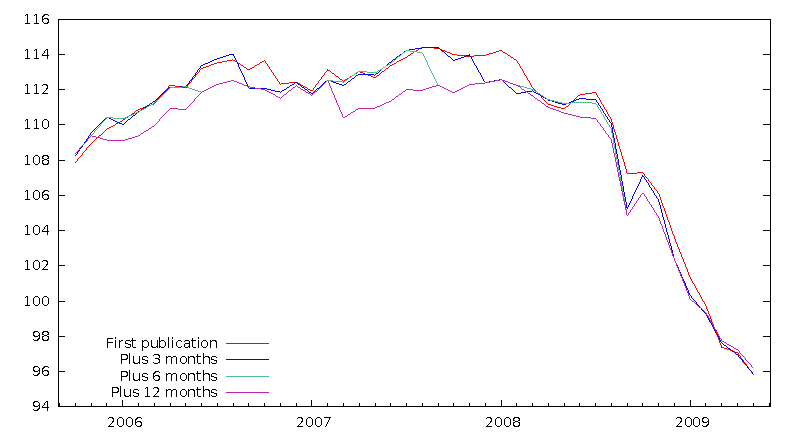
\includegraphics{figures/realtime}
  \caption{Successive revisions to US industrial production}
  \label{fig:realtime-lag}
\end{figure}

\begin{script}[htbp]
  \caption{Retrieving successive realtime lags of US industrial
    production}
  \label{ex:revisions}
\begin{scode}
function series rel_ok (series *obsdate, series *reldate, int p)
  series y_obs, m_obs, y_rel, m_rel, d_rel
  isoconv(obsdate, &y_obs, &m_obs)
  isoconv(reldate, &y_rel, &m_rel, &d_rel)
  series dm = (12*y_rel + m_rel) - (12*y_obs + m_obs)
  return dm < p || (dm == p && d_rel == 1)
end function

nulldata 45
setobs 12 2005:10

string fname = "INDPRO.txt"

# initial published values
join @fname firstpub --data=INDPRO --tkey=observation_date \
--timecols=realtime_start_date --aggr=min(realtime_start_date)

# plus 3 months
join @fname plus3 --data=INDPRO --tkey=observation_date \
--timecols="observation_date,realtime_start_date" \
--filter="rel_ok(&observation_date, &realtime_start_date, 3)" \
--aggr=max(realtime_start_date)

# plus 6 months
join @fname plus6 --data=INDPRO --tkey=observation_date \
--timecols="observation_date,realtime_start_date" \
--filter="rel_ok(&observation_date, &realtime_start_date, 6)" \
--aggr=max(realtime_start_date)

# plus 12 months
join @fname plus12 --data=INDPRO --tkey=observation_date \
--timecols="observation_date,realtime_start_date" \
--filter="rel_ok(&observation_date, &realtime_start_date, 12)" \
--aggr=max(realtime_start_date)

setinfo firstpub --graph-name="First publication"
setinfo plus3 --graph-name="Plus 3 months"
setinfo plus6 --graph-name="Plus 6 months"
setinfo plus12 --graph-name="Plus 12 months"

gnuplot firstpub plus3 plus6 plus12 --time --with-lines \
 --output=realtime.pdf { set key left bottom; }
\end{scode}
\end{script}

\section{Getting the revision history for an observation}
\label{sec:realtime-revhist}

For our final example we show how to retrieve the revision history for
a given observation (again using Alfred data on US industrial
production). In this exercise we are switching the time axis: the
observation period is a fixed point and time is ``vintage
time''. 

A suitable script is shown in Example~\ref{ex:revhistory}.  We first
select an observation to track (January 1970). We start the clock in
the following month, when a data-point for this period was first
published, and let it run to the end of the vintage history (in this
file, March 2013).  Our outer time key is the realtime start date and
we filter on observation date; we name the imported \texttt{INDPRO}
values as \texttt{ip\_jan70}. Since it sometimes happens that more
than one revision occurs in a given month we need to select an
aggregation method: here we choose to take the last revision in the
month.

Recall from section~\ref{sec:realtime-atomic} that Alfred records a
new revision only when the data-point in question actually
changes. This means that our imported series will contain missing
values for all months when no real revision took place. Having checked
for ``holes'' in our file (see section~\ref{sec:realtime-fixed-lag})
and found none, we can apply a simple autoregressive procedure to fill
in the data: each missing value equals the prior non-missing value.

Figure~\ref{fig:realtime-revhist} displays the revision history. Over
this sample period the periodic re-basing of the index overshadows
amendments due to accrual of new information.

\begin{script}[htbp]
  \caption{Retrieving a revision history}
  \label{ex:revhistory}
\begin{scode}
# choose the observation to track here (YYYYMMDD)
scalar target = 19700101

nulldata 518 --preserve
setobs 12 1970:02

join INDPRO.txt ip_jan70 --data=INDPRO --tkey=realtime_start_date \
--timecols=observation_date \
--filter="observation_date==target" --aggr=seq:-1

ip_jan70 = ok(ip_jan70) ? ip_jan70 : ip_jan70(-1)
\end{scode}
\end{script}

\begin{figure}[htbp]
  \centering
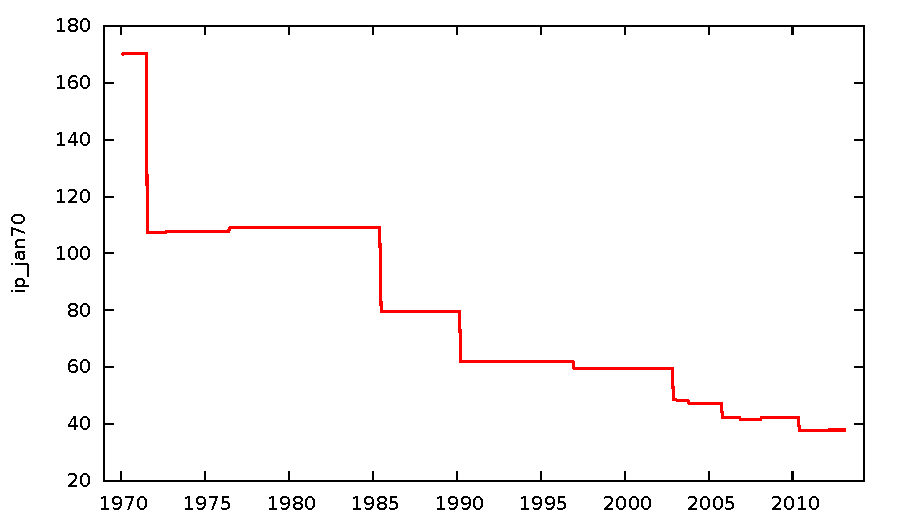
\includegraphics[scale=0.8]{figures/revhist}
\caption{Vintages of US industrial production for January 1970}
  \label{fig:realtime-revhist}
\end{figure}